\section{Proposed simulators}
\label{sec:proposed}

\subsection{Auto-ALS}
\label{sec:auto-als}


\subsection{HeartPole}

\begin{figure}
    \centering
    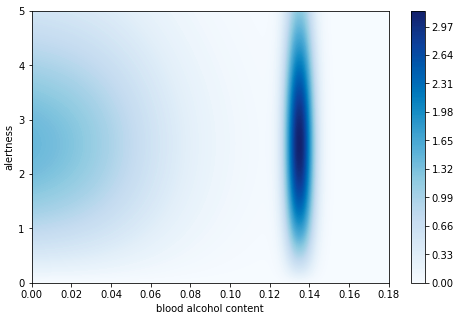
\includegraphics[width=\linewidth]{productivity.png}
    \caption{Productivity function in HeartPole}
    \label{fig:productivity}
\end{figure}%

\begin{figure}
    \centering
    \includegraphics[width=\linewidth]{example.png}
    \caption{An example episode in HeartPole}
    \label{fig:random}
\end{figure}

HeartPole focuses on simplicity and transparency at the expense of realism - it is based on a familiar scenario and a simple set of rules so that when a treatment performs badly it is easy to explore what exactly goes wrong. 
\emph{HeartPole} simulates a creative professional trying to become more productive.
However, many decisions that would help in the short term (not sleeping, consuming coffee and alcohol) can create long-term health issues that negate all short term gains.

In \emph{HeartPole} state $s$ consists of alertness $s^\text{alert}_t$, hypertension $s^\text{hypert}$, intoxication $s^\text{tox}$ time since slept $s^\text{tawake}$, \emph{total time elapsed} $s^\text{ttotal}$ and \emph{total work done} $s^\text{done}$.

Over these parameters, we define \emph{productivity} function $\eta(s^\text{alert}_t, s^\text{tox}_t)$ presented graphically on figure \ref{fig:productivity} and \emph{heart attack probability} $r(s^\text{hypert}_t)=\frac{\text{sigmoid}(s^\text{hypert}_t)}{2}$.
The agent receives small positive rewards for productivity and a very large negative reward if a heart attack occurs.

Every half an hour awake, the agent observes $s_t$ and picks an action $a_t$ from discrete action space of \emph{just work}, \emph{drink coffee} (increases $s^\text{alert}$ and $s^\text{hypert}$), \emph{drink beer} (decreases $s^\text{alert}$, increases $s^\text{hypert}$ and $s^\text{tox}_t$) and \emph{go to bed} (sleep takes a lot of time, but reduces $s^\text{hypert}$ and $s^\text{tox}_t$ and without it alertness starts to fall very fast)

See source code and documentation at \cite{heartpole}.

\subsection{GraphSim}
\label{sec:graphsim}

\begin{figure*}
    \centering
    \includegraphics[width=0.85\linewidth]{graphsim.png}
    \caption{GraphSim}
    \label{fig:graphsim}
\end{figure*}

% Cite mimic3benchmarks

Our last model is trained on MIMIC \cite{mimic} to maximise \emph{accuracy}.
MIMIC can be represented as a set of patients where every patient is an oriented graph, its nodes are patient states, each state is a vector of various clinical measurements, such as blood pressure and oxygen saturation, whereas arcs that connect the patient states are doctors actions, each action a vector of administered drug doses.
These oriented graphs can also be viewed as disjoint clusters in one graph of all possible patient states, a sequence of patient states connected by doctor agents.

\begin{equation}
  G = \{ \langle s_\text{before}, a, s_\text{after} \rangle \}
\end{equation}

Some states in this oriented graph are very similar, it is reasonable to assume that 2 different patients have been in the same state at some point. Our algorithm is based on the idea that if 2 patients have been in the same state, their clinical histories represent 2 possible timelines of events after the state and the choice of timeline depends on doctor's actions.

We find all state pairs $\langle s_A, s_B \rangle$ below a similarity threshold

\begin{equation}
  cos(s_A,s_B) < c_\text{min}
\end{equation}

and merge each into a single state, replacing occurences of $s_A$ and $s_B$ in $G$ with $\frac{s_A+s_B}{2}$. 
The resulting oriented graph becomes the backbone of out simulator.
The simulated patient is initialized in state $s_0$ equal to one of the initial states of real patients in MIMIC.
When at timestep $t$ the agent picks action $a_t$, transition to the next state depends on euclidean distance between the action in the graph and $a_t$ via the softmax function:

\begin{equation}
  p(s_{t+1}|s_t, a_t) = \frac{\sum_{\langle s_\text{before}, a, s_\text{after} \rangle}^G \mathbb{I}[s_\text{before} = s_{t}] \mathbb{I}[s_\text{after} = s_{t+1}] e^{|a_t - a|_2^2}}{\sum_{\langle s_\text{before}, a, s_\text{after} \rangle}^G \mathbb{I}[s_\text{before} = s_{t}]  e^{|a_t - a|_2^2}}
\end{equation}

where $\mathbb{I}$ is the indicator function.

The simulator's source code will be published soon.